% arguelles v2.3.0
% author: Michele Piazzai
% contact: michele.piazzai@uc3m.es
% license: MIT

% Copied from GitHub: https://github.com/piazzai/arguelles

\documentclass[compress,12pt]{beamer}
\usepackage{caption}
\usepackage{subcaption}
\usetheme{Arguelles}

\title{MATH 512 - Project 2}
\subtitle{}
\event{}
\date{}
\author{Wasif Ahmed, Haoxiang Deng, Jacob Fein-Ashley, Kanav Malhotra}


\begin{document}

\frame[plain]{\titlepage}

\Section{Question 1}

\begin{frame}
      \frametitle{Question 1 (a)}
      We use the Kolmogorov-Smirnov test to test for the uniformity of the random numbers generated by the LCG. The test statistic is given by
      \begin{equation*}
            D_n = \max_{1 \leq i \leq n} \left( \frac{i}{n} - U_{(i)} \right) \vee \max_{1 \leq i \leq n} \left( U_{(i)} - \frac{i-1}{n} \right)
      \end{equation*}
      where $U_{(i)}$ is the $i$-th order statistic of the $U_i$'s. 
      
      \begin{itemize}
            \item Our null hypothesis is that the random numbers are uniformly distributed.
            \item  We find that $D_n = 0.0105$ and a p-value of $ 0.208$. This means that we fail to reject the null hypothesis at the 5\% significance level, and conclude that the random numbers are uniformly distributed.
      \end{itemize}
\end{frame}

\begin{frame}
      \frametitle{Question 1 (a)}
      \begin{figure}
            \centering
            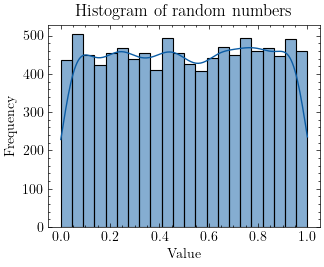
\includegraphics[scale=0.7]{imgs/1a.png}
      \end{figure}
\end{frame}

\begin{frame}
      \frametitle{Question 1 (b)}

      Parameters: $a = 6, m = 11, x_0 = 3, c = 1$
      \begin{itemize}
            \item The sequence is $[3, 7, 9, 10, 5, 8, 4, 2, 1, 6]$
            \item The period is 1
            % \item What do you observe?
      \end{itemize}

      Parameters: $a = 6, m = 10, x_0 = 3, c = 1$
      \begin{itemize}
            \item The sequence is $[3, 8, 8, 8, 8, 8, 8, 8, 8, 8]$
            \item The period is 2
            % \item  What do you observe?
      \end{itemize}

\end{frame}

\begin{frame}
      \frametitle{Question 1 (c)}
      \begin{figure}
            \centering
            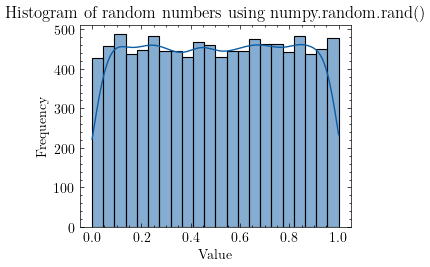
\includegraphics[scale=0.7]{imgs/1d.png}
      \end{figure}
\end{frame}

\begin{frame}
      \frametitle{Question 1 (d)}
      \begin{figure}
            % put the histograms next to each other
            \centering
            \begin{subfigure}{0.45\textwidth}
                  \centering
                  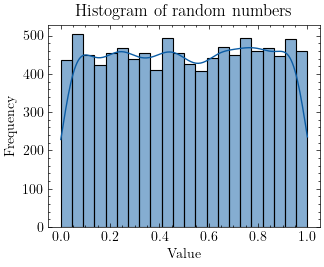
\includegraphics[scale=0.5]{imgs/1a.png}
            \end{subfigure}
            \begin{subfigure}{0.45\textwidth}
                  \centering
                  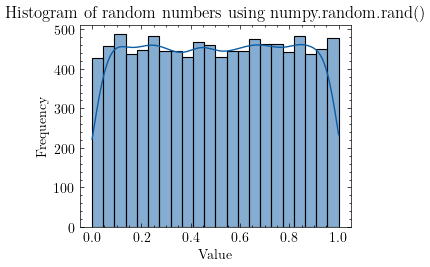
\includegraphics[scale=0.5]{imgs/1d.png}
            \end{subfigure}
      \end{figure}

      \begin{itemize}
            \item The two histograms look relatively similar, meaning both look relatively uniform.
      \end{itemize}
\end{frame}

\begin{frame}
      \frametitle{Question 1 (e)}
      \begin{figure}
            \centering
            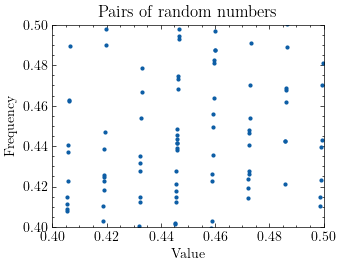
\includegraphics[scale=0.6]{imgs/pairs.png}
      \end{figure}
      \begin{itemize}
            \item I'm not seeing much of a pattern\dots
      \end{itemize}
\end{frame}

\begin{frame}
      \frametitle{Question 1 (f)}
      Disadvantages of LCG:
      \begin{itemize}
            \item It can appear to be random with the right set of parameters, but as we saw, it can get ``stuck'' in a loop.
            \item The randomness depends on the bit position of the seed.
            \item The randomness depends on the choice of parameters.
      \end{itemize}
\end{frame}

\Section{Question 2}
\begin{frame}
      \begin{figure}
            \centering
            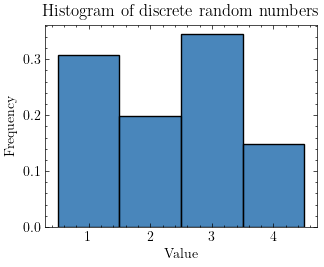
\includegraphics[scale=0.6]{imgs/discrete.png}
      \end{figure}
      
\end{frame}

\End
\begin{frame}[plain,standout]
      \centering
      In combination with \textit{plain}, \\
      it makes a nice thank-you slide!
      \vfill
      \scalebox{4}{\faGithub} \par\bigskip
      \url{https://github.com/piazzai/arguelles} \\
      \url{https://ctan.org/pkg/beamertheme-arguelles}
\end{frame}

\end{document}
